\documentclass[table]{beamer}
% \documentclass[table,handout]{beamer}
% \setbeameroption{show notes}
% \setbeameroption{hide notes}
% \setbeameroption{show only notes}
\usepackage{varwidth}

\newif\ifhide
\newif\ifpost
\newif\ifhideclicker

\hidetrue
% \hideclickertrue
% \posttrue

\newcommand{\whiteout}[1]{\textcolor{white}{#1}}
\newcommand{\whiteoutbox}[1]{\fcolorbox{white}{white}{\parbox{\dimexpr \linewidth-2\fboxsep-2\fboxrule}{\whiteout{#1}}}}
\newcommand{\notebox}[1]{\fcolorbox{blue}{white}{\parbox{\dimexpr \linewidth-2\fboxsep-2\fboxrule}{#1}}}

\ifhide%
    \newcommand{\hmask}[1]{\phantom{\varwidth{\linewidth}#1\endvarwidth}}%
\else%
    \newcommand{\hmask}[1]{#1}%
\fi

\ifhide%
    \newcommand{\hignore}[1]{}%
\else%
    \newcommand{\hignore}[1]{#1}%
\fi

\ifpost%
    \newcommand{\nopost}[1]{}%
\else%
    \newcommand{\nopost}[1]{#1}%
\fi

\ifhide%
    \newcommand{\hidebox}[1]{\phantom{\varwidth{\linewidth}#1\endvarwidth}}%
\else%
    \newcommand{\hidebox}[1]{\fbox{\parbox{\linewidth}{#1}}}%
\fi

\ifhide%
    \newcommand{\wbox}[1]{\whiteoutbox{#1}}%
\else%
    \newcommand{\wbox}[1]{\notebox{#1}}%
\fi

% \ifhide%
%     \newcommand{\clickeranswer}[1]{#1}%
% \else%
%     \newcommand{\clickeranswer}[1]{\textbf{\textcolor{blue}{#1}}}%
% \fi

\ifhideclicker%
    \newcommand{\clickeranswer}[1]{#1}%
\else%
    \ifhide%
        \newcommand{\clickeranswer}[1]{#1}%
    \else%
        \newcommand{\clickeranswer}[1]{\textbf{\textcolor{blue}{#1}}}%
    \fi
\fi

\input{../utils/slide-preamble2.tex}
\newcommand{\highlight}[1]{\textcolor{violet}{\textit{\textbf{#1}}}}
\newcommand{\super}[1]{\ensuremath{^{\textrm{#1}}}}
\newcommand{\sub}[1]{\ensuremath{_{\textrm{#1}}}}
\newcommand{\dC}{\ensuremath{^\circ{\textrm{C}}}}
\newcommand{\tb}{\hspace{2em}}
\providecommand{\e}[1]{\ensuremath{\times 10^{#1}}}
\newcommand{\myHangIndent}{\hangindent=5mm}

\makeatletter
\newcommand*{\rom}[1]{\expandafter\@slowromancap\romannumeral #1@}
\makeatother

\newcommand{\blankslide}{{\setbeamercolor{background canvas}{bg=black}
\setbeamercolor{whitetext}{fg=white}
\begin{frame}<handout:0>[plain]
\end{frame}}}

\newcommand{\whiteslide}{
\begin{frame}<handout:0>[plain]
\end{frame}}

\newcommand{\f}[1]{\ensuremath{F_{#1}}}

\bibliography{../bib/references}
\input{../utils/title-info.tex}

\title[Mutualism]{Mutualism}
% \date{\today}
\date{May 26, 2015}

% \setbeamertemplate{section in toc}[sections numbered]
% \setbeamertemplate{subsection in toc}[subsections numbered]

\begin{document}

\begin{noheadline}
\maketitle
\end{noheadline}

\nopost{
\begin{noheadline}
\begin{frame}[c]
    \vspace{-6mm}
    \begin{center} 
        \includegraphics[height=1.2\textheight]{../images/seating-chart-2.pdf}
    \end{center}
\end{frame}
\end{noheadline}
}

\clickerslide{
\begin{noheadline}
\begin{frame}
    \begin{clickerquestion}
        \item Tobacco plants produce nicotine as a defense against
            caterpillars. On average, individuals that are induced to produce
            more nicotine make fewer seeds than non-induced individuals. Why is
            there a cost of defense from consumers---meaning, a fitness
            trade-off?
 
        \begin{clickeroptions}
            \item \clickeranswer{Resources committed to defense can't be used
                    for growth or reproduction.}
            \item It is difficult to produce both standing and induced
                defenses.
            \item Hosts and consumers have coevolved.
            \item Induced defenses are more efficient than standing defenses
                energetically, but take time to produce.
        \end{clickeroptions}
    \end{clickerquestion}
\end{frame}
\end{noheadline}
}

\clickerslide{
\begin{noheadline}
\begin{frame}
    \begin{clickerquestion}
        \item According to the tobacco data you reviewed, there did NOT appear
            to be a cost of defense in tobacco plants that had experienced
            intense selection by herbivores. How could this be? 
 
        \begin{clickeroptions}
            \item It is difficult to produce standing AND induced defenses.
            \item Hosts and consumers have coevolved.
            \item Induced defenses are more efficient than standing defenses
                energetically, but take time to produce.
            \item \clickeranswer{In some cases, plants that are stressed throw
                    all of their remaining resources into reproduction.}
            \item Resources committed to defense can’t be used for growth or
                reproduction.
        \end{clickeroptions}
    \end{clickerquestion}
\end{frame}
\end{noheadline}
}


\begin{noheadline}
\begin{frame}
\frametitle{Today's issues:}
\vspace{5mm}
% \tableofcontents[subsectionstyle=hide]
\tableofcontents
\end{frame}
\end{noheadline}

\section{Treehoppers and ants}

\begin{frame}
    \begin{adjustwidth}{-2em}{-1.5em}
        Recall the treehopper-ant interaction data from the reading

        \begin{itemize}
            \item Why is this interaction ``contingent?''

            \nbox{This mutualistic interaction is contingent upon the density
                of spiders. If there are many spiders around, the fitness of
                both the ants and the hoppers increase. But, if spiders are
                scarce, the interaction becomes parasitic; the ants are
                benefiting from the honeydew, but the hoppers are not gaining
                the benefit of protection to offset the fitness cost of
                producing the honeydew.}
        \end{itemize}
    \end{adjustwidth}
\end{frame}

\clickerslide{
\begin{frame}
    \begin{clickerquestion}
        \item Consider the treehopper-ant interaction data (from the reading).
            Long-term, how would the nature of the interaction change if spider
            density were low every year and ``honeydew'' production is
            expensive?
        \begin{clickeroptions}
            \item \clickeranswer{Selection should favor treehoppers that don't
                    release honeydew.}
            \item Selection should favor ants that eat treehoppers.
            \item Selection should favor treehoppers that eat ants.
            \item Ant populations increase (no energy spent defending against
                spiders).
        \end{clickeroptions}
    \end{clickerquestion}

\end{frame}
}

\section{Mycorrhizal and endophytic fungi}

\begin{frame}
    \begin{adjustwidth}{-2em}{-1.5em}
        \begin{columns}

            \column{0.5\linewidth}

            Mycorrhizal fungi

            \vspace{4mm}
            Fungi growing on roots of plants

            \vspace{4mm}
            What do you notice about this photograph?

            \nbox{LOTS of fungi, relatively small amount of plant root biomass.
                Also, fungi are connecting the roots of different seedlings.}

            \column{0.49\linewidth}

            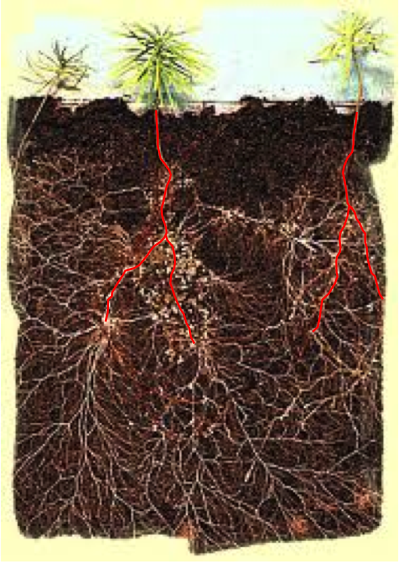
\includegraphics[width=\columnwidth]{roots.png}

        \end{columns}
    \end{adjustwidth}
\end{frame}

\section{Nitrogen-fixing bacteria}

\section{Ants that farm fungi}

\section{Pollination}

\end{document}

\clickerslide{
\begin{frame}
    \begin{clickerquestion}
        \item 
        \begin{clickeroptions}
            \item 
            \item 
            \item 
            \item 
        \end{clickeroptions}
    \end{clickerquestion}
\end{frame}
}

\clickerpost{
{
\usebackgroundtemplate{\includegraphics[page=17,width=\paperwidth]{./24-Radiation-extinction.pdf}}
\begin{frame}[t,plain]
    \begin{adjustwidth}{-2em}{-1.5em}
        \cmask{Answer: 3}
    \end{adjustwidth}
\end{frame}
}
}

